\documentclass[11pt,a4paper]{article}
\usepackage[utf8]{inputenc}
\usepackage{amsmath}
\usepackage{amsfonts}
\usepackage{amssymb}
\usepackage[left=2cm,right=2cm,top=2cm,bottom=2cm]{geometry}


\usepackage{slashed}
\usepackage{hyperref}
\usepackage{graphicx}
\usepackage{caption}
\usepackage{float}
\usepackage{subcaption}
\usepackage{multirow}
\usepackage{minted}
\usepackage[dvipsnames]{xcolor}


\renewcommand{\theequation}{\arabic{section}.\arabic{equation}}



\usepackage{ifthen}
\usepackage[dvipsnames]{xcolor}
\usepackage{tikz}


%Define color environments:

\newenvironment{DK}[1]{{\color{gray}Commend from D: #1}}

\newenvironment{DKnew}[1]{{\color{blue}NEW from D: #1}}

\newenvironment{DKres}[1]{{\color{BrickRed}RESTRUCTURED from D: #1}}




\newcommand{\dint}{  \displaystyle \int }
%%%%%%%%%%%%%%%%%%%%%%%%%%%%%%%%%%%%%%%%%%
\newcommand{\ie}{{\em i.e.} }
\newcommand{\eg}{{\em e.g.} }
\newcommand{\GeV}{{\rm GeV}}
\newcommand{\TeV}{{\rm TeV}}
\newcommand{\MeV}{{\rm MeV}}
\newcommand{\keV}{{\rm keV}}

\newcommand{\rhs}{RHS }
\newcommand{\lhs}{LHS }


\newcommand{\geff}{ g_{\rm eff} }
\newcommand{\heff}{ h_{\rm eff} }
 
\newcommand{\Ham}{ \mathcal{H} }
 
\newcommand{\thetamax}{ \theta_{\rm max}{} }

 
\newcommand{\thetai}{ \theta_{\rm ini}{} }

\newcommand{\fa}{ f_{\alpha}{} }
 
\newcommand{\ti}{ t_{\rm ini}{} }
 
\newcommand{\Ri}{ R_{\rm ini}{} }


\newcommand{\tosc}{ t_{\rm osc}{} }

\newcommand{\Omegai}{ \Omega_{\rm ini} }
 
\newcommand{\ma}{ m_\alpha{} }

\newcommand{\Lint}{ \mathcal{L}_{\rm int} }


\newcommand{\vev}[1]{\langle #1 \rangle}
\newcommand{\Bvev}[1]{\Bigg\langle #1 \Bigg\rangle}
\newcommand{\bvev}[1]{\Big\langle #1 \Big\rangle}




\newcommand{\lrb}[1]{\left( #1 \right)}
\newcommand{\lrsb}[1]{\left[ #1 \right]}
\newcommand{\lrBigb}[1]{\Big( #1 \Big)}
\newcommand{\lrBigsb}[1]{\Big[ #1 \Big]}
\newcommand{\lrBiggb}[1]{\Bigg( #1 \Bigg)}
\newcommand{\lrBiggsb}[1]{\Bigg[ #1 \Bigg]}

\newcommand{\lrBigcb}[1]{\Big\{ #1 \Big\}}
\newcommand{\lrBiggcb}[1]{\Bigg\{ #1 \Bigg\}}
%%%%%%%%%%%%%%%%%%%%%%%%%%%%%%%%%%%%%%%%%

%%%%%%%%%%%%%%%%%%%%%%%%%%%%%%%%%%%%%%%%%%%%%%%%%%%--Begin_refs--%%%%%%%%%%%%%%%%%%%%%%%%%%%%%%%%%%%%%%%%%%%%%%%%%%%%%%%%%%%%%%%%%%%%%%
\newcounter{NumArgs}

%Define reference to an arbitrary number of equations (\eqs{label_1,label_2....,label_n} will show eqs. ref_1, ref_2, ..., and ref_n)
\newcommand{\eqs}[1]{\setcounter{NumArgs}{0}\foreach\i in{#1}{\stepcounter{NumArgs}}%
\ifthenelse{\equal{\theNumArgs}{1}}{eq.~(\ref{#1})}%
{\ifthenelse{\equal{\theNumArgs}{2}}%
{eqs.~\foreach\i[count=\q]in{#1}{\ifthenelse{\equal{\q}{\theNumArgs}}{and (\ref{\i})}{(\ref{\i})~}}}%
{eqs.~\foreach\i[count=\q]in{#1}{\ifthenelse{\equal{\q}{\theNumArgs}}{and (\ref{\i})}{(\ref{\i}),~}}}}}


%Define reference to an arbitrary number of equations (\Eqs{label_1,label_2....,label_n} will show Eqs. ref_1, ref_2, ..., and ref_n)
\newcommand{\Eqs}[1]{\setcounter{NumArgs}{0}\foreach\i in{#1}{\stepcounter{NumArgs}}%
\ifthenelse{\equal{\theNumArgs}{1}}{Eq.~(\ref{#1})}%
{\ifthenelse{\equal{\theNumArgs}{2}}%
{Eqs.~\foreach\i[count=\q]in{#1}{\ifthenelse{\equal{\q}{\theNumArgs}}{and (\ref{\i})}{(\ref{\i})~}}}%
{Eqs.~\foreach\i[count=\q]in{#1}{\ifthenelse{\equal{\q}{\theNumArgs}}{and (\ref{\i})}{(\ref{\i}),~}}}}}


%Define reference to an arbitrary number of labels (\REF{label_1,label_2....,label_n} will show ref_1, ref_2, ..., and ref_n)
\newcommand{\refs}[1]{\setcounter{NumArgs}{0}\foreach\i in{#1}{\stepcounter{NumArgs}}%
\ifthenelse{\equal{\theNumArgs}{1}}{(\ref{#1})}%
{\ifthenelse{\equal{\theNumArgs}{2}}%
{\foreach\i[count=\q]in{#1}{\ifthenelse{\equal{\q}{\theNumArgs}}{and (\ref{\i})}{(\ref{\i})~}}}%
{\foreach\i[count=\q]in{#1}{\ifthenelse{\equal{\q}{\theNumArgs}}{and (\ref{\i})}{(\ref{\i}),~}}}}}



%Define reference to an arbitrary number of figs (\Figs{label_1,label_2....,label_n} will show ref_1, ref_2, ..., and ref_n)
\newcommand{\Figs}[1]{\setcounter{NumArgs}{0}\foreach\i in{#1}{\stepcounter{NumArgs}}%
\ifthenelse{\equal{\theNumArgs}{1}}{Fig.~(\ref{#1})}%
{\ifthenelse{\equal{\theNumArgs}{2}}%
{Figs.~\foreach\i[count=\q]in{#1}{\ifthenelse{\equal{\q}{\theNumArgs}}{and (\ref{\i})}{(\ref{\i})~}}}%
{Figs.~\foreach\i[count=\q]in{#1}{\ifthenelse{\equal{\q}{\theNumArgs}}{and (\ref{\i})}{(\ref{\i}),~}}}}}




%Define reference to an arbitrary number of "general reference" (\Gen{message}{label_1,label_2....,label_n} will show message.(ref_1), (ref_2), ..., and (ref_n)
\newcommand{\Gen}[2]{\setcounter{NumArgs}{0}\foreach\i in{#2}{\stepcounter{NumArgs}}%
	\ifthenelse{\equal{\theNumArgs}{1}}{#1.~(\ref{#2})}%
	{\ifthenelse{\equal{\theNumArgs}{2}}%
		{#1.~\foreach\i[count=\q]in{#2}{\ifthenelse{\equal{\q}{\theNumArgs}}{and (\ref{\i})}{(\ref{\i})~}}}%
		{#1.~\foreach\i[count=\q]in{#2}{\ifthenelse{\equal{\q}{\theNumArgs}}{and (\ref{\i})}{(\ref{\i}),~}}}}}


%%%%%%%%%%%%%%%%%%%%%%%%%%%%%%%%%%%%%%%%%%%%%%%%%%%--End_refs--%%%%%%%%%%%%%%%%%%%%%%%%%%%%%%%%%%%%%%%%%%%%%%%%%%%%%%%%%%%%%%%%%%%%%%



%%%%%%%-----------------------Rules-----------------------%%%%%%%
% 1. Put any new macros in macros.tex.

% 2. Section should start with:
	%\section{This is a section}\label{sec:Intro}
	%\setcounter{equation}{0}

% 3. labels for Figs should start with fig:, for equations should start with eq:, for sections with sec:, etc.
%%%%%%%--------------------------------------------------%%%%%%%




\author{Karamitros Dimitrios}
\title{{\tt MiMeS}: Misalignment Mechanism Solver}
\begin{document}

\maketitle

\begin{abstract}
	We introduce a \CPP header-only library that solves the Axion equation of motion, \mimes.  
	\mimes makes no assumptions regarding the cosmology and the thermal mass of the axion, which allows the user 
	to consider various cosmological scenarios and axion-like models.
	Moreover, although written entirely in \CPP, \mimes comes with a convenient \PY interface, which, at most, 
	only requires by the user to write a few lines of elementary code in \CPP.
\end{abstract}


\section{Introduction}\label{sec:intro}
\setcounter{equation}{0}

About the axion...

\section{Physics background}\label{sec:abundance}
\setcounter{equation}{0}
%
Although there are several works in the literature (such as~\cite{Chang:1998ys}) that can provide a insight on the solution of the axion equation of motion (EOM), in this section we define, derive, and discuss the various quantities we need, in order to understand how \mimes works in detail.

\paragraph{The EOM} %The axion field is written as 
%
%\begin{equation}
%	A  \equiv \fa \ \theta,
%	\label{eq:fa_def}
%\end{equation}
%%
%with $\fa$ the scale of the axion that determines the the scale at which the PQ symmetry breaks. 
%
The EOM in terms of the axion angle, $\theta$, is 
%
\begin{equation}
	\lrb{\dfrac{d^2}{d t^2} + 3 H(t) \ \dfrac{d}{d t} } \theta(t) + \maT^2(t) \ \sin \theta(t) = 0 \; ,
	\label{eq:eom}
\end{equation}
%
with $H(t)$ the Hubble parameter (determined by the cosmology), and $\maT(t)$  the time (temperature) dependent mass of the axion, with 
\begin{equation}
	\maT^2(T) = \dfrac{\chi(T)}{\fa^2}\;,
	\label{eq:axion_mass_def}
\end{equation} 
%
and $\chi$ a function of the temperature, and $\fa$ the scale at which the Peccei Quinn symmetry breaks \DK{ref??}. For the QCD axion, this has been calculated using lattice simulations in~\cite{Borsanyi:2016ksw}.~\footnote{The data provided by ref.~\cite{Borsanyi:2016ksw} are used by  \mimes out-of-the-box. However, the user is free to change them.}


\paragraph{Initial conditions}
%
\begin{figure}[h!]
	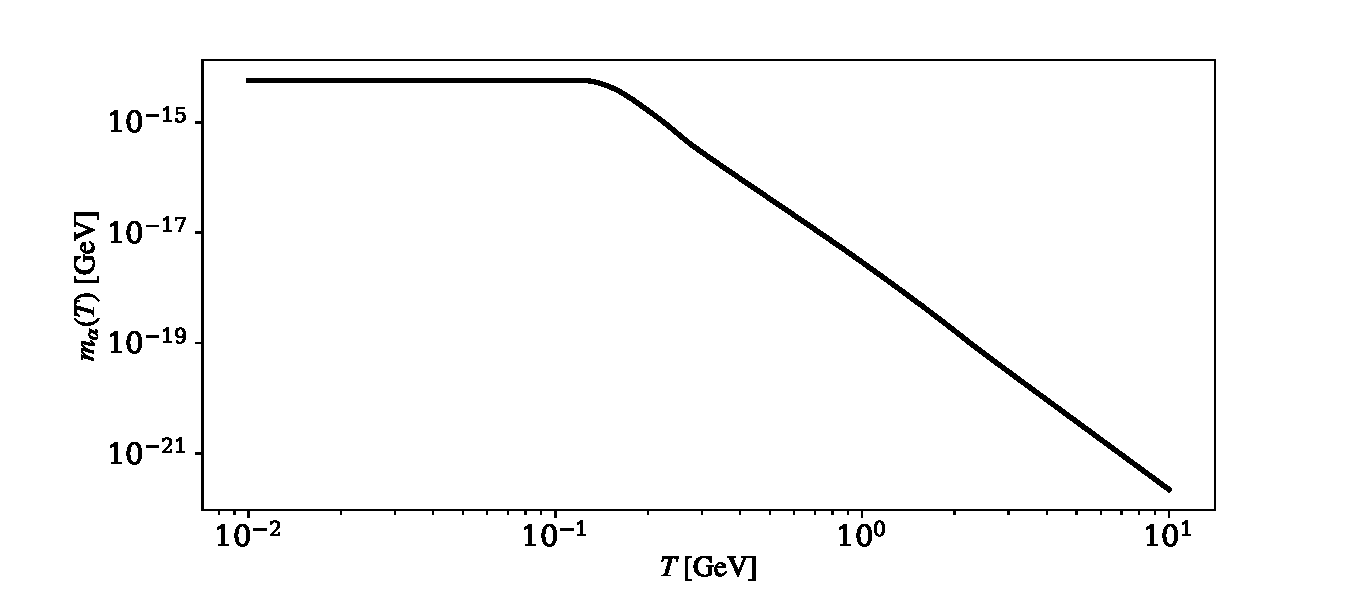
\includegraphics[width=1\textwidth]{figs/axion_mass.pdf}
	\caption{The mass of the axion as a function of the temperature for $\fa=10^{12}~\GeV$, using the data provided in ref.~\cite{Borsanyi:2016ksw}.}
	\label{fig:axion_mass}
\end{figure}
%
Assuming that the PQ symmetry breaks before inflation, the initial conditions (\ie at some $t=0$, after inflation) for the EOM is random. However, we note that $\maT \to 0$ (see \Figs{fig:axion_mass}) -- \ie $\maT \ll H$ -- at very early times. Therefore, after inflation, the EOM is simply
%
\begin{equation}
	\lrb{\dfrac{d^2}{d t^2} + 3 H(t) \ \dfrac{d}{d t}  } \theta(t) = 0 \; ,
	\label{eq:massless_eom}
\end{equation}
%
which is solved by $\theta = \thetai + C \dint_{0}^t d t' \ \lrb{ \dfrac{a(t'=0)}{a(t')} }^3$, with $\thetai$ a constant and $a$ the scale factor of the Universe. That is, as the Universe expands, $\theta \approx \thetai$. Since we would like to calculate the relic abundance of axions, we can integrate \eqs{eq:eom} from a time after inflation (call it $t = \ti$) such that $ \dot \theta |_{t=\ti} = 0$ and  $\theta|_{t=\ti} \approx \thetai$.   



\subsection{The WKB approximation}
%
In order to solve analytically \eqs{eq:eom}, we assume $\theta \ll 1$, which results in the linearised EOM
%
\begin{equation}
	\lrb{\dfrac{d^2}{d t^2} + 3 H(t) \ \dfrac{d}{d t} + \maT^2(t) } \theta(t) = 0 \; .
	\label{eq:linear_eom}
\end{equation}

Using a trial solution $\theta_{\rm trial} = \exp\lrsb{ i \dint d t \ \lrBigb{u(t) +3/2 \ i \ H(t)} }$, and defining $\Omega^2 = \maT^2 - \dfrac{9}{4} H^2 -  \dfrac{3}{2} \dot H $ we can transform the \eqs{eq:linear_eom} to 
%
\begin{equation}
	u^2 = \Omega^2 + i \ \dot u \; ,
	\label{eq:eom_of_u}
\end{equation}
%
which has a formal solution $u = \pm \sqrt{\Omega^2 + i \dot u}$. Assuming that $\dot u \ll \Omega^2$ and $\dot \Omega \ll \Omega^2$, we can approximate $u$ as
%
\begin{equation}
	u \approx \pm \Omega + \dfrac{i}{2} \dfrac{d \log \Omega}{d t} \;,
	\label{eq:u_approx}
\end{equation}
%
which results in the general solution of \eqs{eq:linear_eom} 
%
\begin{equation}
	\theta \approx \dfrac{1}{\sqrt{\Omega}} \exp\lrb{-\dfrac{3}{2} \int d t \ H} \lrsb{ A \cos\lrb{ \int d t \ \Omega} +  B \sin\lrb{ \int d t \ \Omega}    } \;. 
	\label{eq:general_solution_eom_approx}
\end{equation}

Applying, then, the initial conditions $ \dot \theta |_{t=\ti} = 0$ and  $\theta|_{t=\ti} \approx \thetai$, we arrive at 
%
\begin{equation}
\theta(t) \approx \thetai \sqrt{ \dfrac{ \Omegai }{\Omega (t)} } \lrb{\dfrac{a}{\ai}}^{-3/2} \  \cos\lrb{ \int_{\ti}^t d t^\prime  \ \Omega(t^\prime)}   \;.
\label{eq:solution_eom_approx} 
\end{equation}


In order to further simplify this approximate result, we note that $\theta$ deviates from $\thetai$ close to $t=\tosc$ -- corresponding to $T = \Tosc$, the so-called ``oscillation temperature" -- $\maT|_{t = \tosc} = 3 H|_{t = \tosc}$, which is defined as the point at which the axion begins to oscillate. 
%
This observation allows us to set $\ti = \tosc$.  Moreover, at $t > \tosc$, we approximate $\Omega \approx \maT$, as $H^2$ and $\dot H$ become much smaller than $\maT^2$ quickly after $t=\tosc$. Finally, the axion angle takes the form
%
\begin{equation}
	\theta(t) \approx \thetaosc \lrb{\dfrac{3}{4}}^{1/4} \sqrt{ \dfrac{ \maT|_{t=\tosc} }{\maT  (t)} } \lrb{\dfrac{a}{\aosc}}^{-3/2} \  \cos\lrb{ \int_{\tosc}^t d t^\prime  \ \maT(t^\prime)}   \;,
	\label{eq:solution_eom_approx_theta_osc} 
\end{equation}
%
where $\thetaosc = \theta|_{t=\tosc}$. This equation is further simplified if we assume that $\thetaosc \approx \thetai$, \ie
%
\begin{equation}
	\theta(t) \approx \thetai \lrb{\dfrac{3}{4}}^{1/4} \sqrt{ \dfrac{ \maT|_{t=\tosc} }{\maT  (t)} } \lrb{\dfrac{a}{\aosc}}^{-3/2} \  \cos\lrb{ \int_{\tosc}^t d t^\prime  \ \maT(t^\prime)}   \;.
	\label{eq:solution_eom_approx_final} 
\end{equation}
%
It is worth mentioning that the accuracy of this approximation depends, in general, on $\Tosc$; it determines the difference between $\thetai$ and $\thetaosc$, the deviation of $\dot \theta|_{t=\tosc}$ from $0$, and whether $\dot \Omega \ll \Omega^2$. 


\paragraph{Axion energy density}
%
The energy density of the axion is 
%
\begin{eqnarray}
	\rho_{a} = \dfrac{1}{2} \fa^2 \lrsb{ \dot{\theta}^2 + \maT^2 \theta^2 } \;.
	\label{eq:rho_a_def} 
\end{eqnarray}
%
For the relic abundance of axions, we need to calculate their energy density at very late times. That is, $\dot{\tilde{m}}_a = 0$, $\maT \gg H$ and $\dot H \ll H^2$. After some algebra, we obtain the approximate form of the energy density (as a function of the scale factor $a$) 
%
\begin{eqnarray}
	\rho_{a} \approx \dfrac{\ma }{2}  \ \fa^2 \ \thetai^2  \ \maT(\aosc) \ \lrb{\dfrac{\aosc}{a}}^3 \;,
	\label{eq:rho_a0} 
\end{eqnarray}
%
which shows that the energy density of axions at late times scales as the energy density of matter. If there is a period of entropy injection to the plasma for $T<\Tosc$, the axion energy density gets diluted, since 
%
\begin{equation}
	a^3 \ s = \gamma \ \aosc^3 \ s_{\rm osc} \Rightarrow  \lrb{\dfrac{\aosc}{a}}^3 = \gamma^{-1} \dfrac{s}{s_{\rm osc}} \;,
\end{equation}
%
with $\gamma$ the amount of entropy injection to the plasma between $\tosc$ and $t$. Therefore, the present (at $T=T_0$) energy density of the axion, becomes
%
\begin{eqnarray}
	\rho_{a,0} = \gamma^{-1}  \dfrac{s_0}{s_{\rm osc}} \  \dfrac{1 }{2}  \ \fa^2 \ \ma \ \maT_{,{\rm osc}} \ \thetai^2    \;,
	\label{eq:rho_a_approx} 
\end{eqnarray}
with $\ma$ the mass of the axion at $T=T_0$. Notice that the explicit dependence on $\fa$ cancels, since $\maT \sim 1/\fa$. That is, $\fa$ only affects the energy density of the axions through its impact on $\Tosc$. 
%

\subsection{Notation}\label{sec:notation}
%
%The WKB approximation is very useful in order to understand the evolution of the axion field. However, it fails to explain how the oscillation begins before $\dot \Omega \ll \Omega^2$ is reached. In this section we will try to understand the evolution of the axion as generally as possible. 
%
The EOM~(\ref{eq:eom}) depends on time, which is not very useful variable in a non-standard comsological setting. Therefore, we introduce 
%
\begin{eqnarray}
	u = \log \dfrac{a}{\ai} \;,
	\label{eq:natation}
\end{eqnarray}
%
which results in 
%
\begin{eqnarray}
	&\dfrac{d F}{dt} &=  H  \dfrac{d F}{du} 
	\nonumber \\
	&\dfrac{d^2 F}{dt^2} &= H^2 \ \lrb{ \dfrac{d^2 F}{du^2} + \dfrac{1}{2} \dfrac{d \log H^2}{du}  \dfrac{d F}{du} }\;.
	\label{eq:deriv_u}
\end{eqnarray}

The EOM in terms of $u$, then, becomes
%
\begin{equation}
	\dfrac{d^2  \theta}{du^2} + \lrsb{\dfrac{1}{2} \dfrac{d \log H^2}{du} + 3 } \dfrac{d  \theta}{d u} + \ \lrb{\dfrac{\maT}{H}}^2 \ \sin \theta
	=0 \;.
	\label{eq:eom_u}
\end{equation}

Notice that in a radiation dominated Universe
%
$$
\dfrac{d \log H^2}{du} = -\lrb{ \dfrac{d \log \geff}{d \log T} +4 } \delta_h^{-1}\;,
$$
with  $ \delta_h = 1+ \dfrac{1}{3} \dfrac{d \log \heff}{d \log T} $. 
%
In a general cosmological setting, the expansion rate is dominated by an energy density that scales as $\rho \sim a^{-c}$, which results in $\dfrac{d \log H^2}{du}  = -c$. However, close to rapid particle annihilations and decays, the evolution of the energy densities change, and $\dfrac{d \log H^2}{du}$ can only be computed numerically.

\subsection{Beyond the WKB approximation}\label{sec:beyond_WKB}
%
The WKB approximation is very useful, as it helps us understand the evolution of the axion field after it begins to oscillate adiabatically. However, it fails to capture the dynamics the adiabatic conditions are met, result in inaccurate axion relic abundance result. In this section, we examine the deviation of $\thetaosc$ from the initial value of $\theta$, as well how to treat cases where the EOM cannot be linearized.

\subsubsection{Behaviour close to the initial condition}\label{sec:close_to_ini}
%
The accuracy of the approximate evolution of the axion angle given in \eqs{eq:solution_eom_approx_final} depends on the deviation between $\thetai$ and $\thetaosc$. In order to examine their deviation, we expand \eqs{eq:eom} at a time $t =\ti + \delta t$ with $\delta t \to 0$. That is, we use the following approximations 
%
\begin{equation*}
	\ddot{\theta} \approx \dfrac{\dot \theta (\ti+ \delta t)  - \dot \theta (\ti)}{ \delta  t } =  \dfrac{\dot \theta (\ti + \delta t)  }{\delta  t } \;,
	\qquad
	\dot \theta(\ti + \delta t) = \dfrac{\theta(\ti + \delta t) - \thetai}{\delta t} \;.
\end{equation*} 
%
and, solve the EOM~\ref{eq:eom} for $\theta(\ti + \delta t)$. This results in
%
\begin{equation}
	\theta(\ti + \delta t)  \approx  \thetai -\dfrac{\delta t^2}{1+3\ \delta t \ H(\ti + \delta t) } \  \maT^2(\ti + \delta t)  \sin \theta(\ti + \delta t)  
	\approx   \thetai - \delta t^2 \ \maT^2(\ti) \ \sin \thetai  \ + \mathcal{O}(\delta t^3)\;, 
	\label{eq:theta_dt}
\end{equation}
%
which indicates that the angle decreases (increases) as the temperature drops if $\thetai>0$ ($\thetai<0$). Using the notation introduced in section~\ref{sec:notation}, \eqs{eq:theta_dt} takes the form
%
\begin{eqnarray}
	\theta \approx    \thetai - \delta u^2 \ \lrb{\dfrac{\maT}{H}}_{t=\ti}^2 \ \sin \thetai \;,
	\label{eq:theta_du}
\end{eqnarray}
%
which can be used to estimate the angle at the oscillation temperature
%
\begin{eqnarray}
	\thetaosc \approx    \thetai -  \lrb{\dfrac{\maT}{H}}_{t=\ti}^2 
	\lrsb{1- \dfrac{\Ti}{\Tosc}\lrb{\dfrac{\heff_{,\rm ini}}{\heff_{,\rm osc}}\gamma_{\rm osc}}^{1/3}}^{2}   \ \sin \thetai \;,
	\label{eq:theta_osc}
\end{eqnarray}
%
where  $\gamma_{\rm osc}$ is the entropy injection between $\Ti$ and $\Tosc$. Notice that in the derivation of \eqs{eq:solution_eom_approx_final} we used $\theta_{\rm osc} = \thetai$ as our first approximation. Thus, \eqs{eq:theta_osc} provides a correction that takes into account the deviation between $\theta_{\rm osc} $ and $ \thetai$, and \eqs{eq:rho_a_approx} becomes (for $\thetai \ll 1$)
%
\begin{eqnarray}
	\rho_{a,0} = \gamma^{-1}  \dfrac{s_0}{s_{\rm osc}} \  \dfrac{1 }{2}  \ \fa^2 \ \ma \ \maT_{,{\rm osc}} \ \thetai^2 \lrBiggcb{
		1 - \ \lrb{\dfrac{\maT}{H}}_{t=\ti}^2 \  \lrb{1- \dfrac{\Ti}{\Tosc}\lrb{\dfrac{\heff_{,\rm ini}}{\heff_{,\rm osc}}\gamma_{\rm osc}}^{1/3}}^{2}   }^2    \;,
	\label{eq:rho_a_NLO} 
\end{eqnarray}
%
which implies that the WKB approximation overestimates the energy density of the axion, since $\gamma_{\rm osc}$, $H_{\rm ini}$, and $\Tosc$ can vary. 


In order to demonstrate the effect of the deviation between $\thetai$ and $\thetaosc$, we show \Figs{fig:WKB_diff_i,fig:WKB_diff_osc}, for different cosmological scenarios. In both figures, the red and black (dashed) lines correspond to radiation and matter dominated Universe, respectively.~\footnote{For the matter dominated case (following the notation of refs.~\cite{Arias:2019uol,Arias:2020qty}), we have used 
$T_{\rm end}=10^{-2} ~\GeV,\; c=3, \; T_{\rm ini}=10^{12} ~\GeV, \; \text{and}\; r=0.1$.} For the matter dominated case, entropy is injected to the plasma both before and after $\Tosc$. The entropy injection factor, $\gamma_{\rm osc}$, as a function of $\fa$ is shown in \Figs{fig:gamma_osc}.

In \Figs{fig:WKB_diff_i} we show the relative difference between $\Omega h^2$ using \eqs{eq:solution_eom_approx_final} and the result obtained from \mimes. It should be apparent that the accuracy of the estimate based on \eqs{eq:solution_eom_approx_final} depends of $\fa$, since for high values of $\fa$, $\Tosc$ is low. That is, the deviation between $\thetai$ and $\thetaosc$ is greater than the corresponding difference for lower $\fa$, especially for the matter dominated case, where the entropy injection is great (see \Figs{fig:gamma_osc}).

In \Figs{fig:WKB_diff_osc} we show the relative difference between $\Omega h^2$ obtained by integrating numerically \eqs{eq:eom_u}  and using \eqs{eq:solution_eom_approx_theta_osc} with \eqs{eq:theta_osc}. The relative difference between the two estimates, once again, depends $\fa$. It should be noted that the estimate for $\thetaosc$ depends on the choice of $\Ti$. For \Figs{fig:WKB_diff_osc}, we define $\Ti$ as the temperature at which $3H/\maT = 2$. We note that this estimate is more accurate, its accuracy still depends on whether the axion evolves adiabatically at $T<\Tosc$. Moreover, an increase of $\gamma_{\rm osc}$ invalidates the estimate of $\thetaosc$; higher powers of $\delta u$ may be needed.    
%
\begin{figure}[t]
	\begin{subfigure}[]{0.5\textwidth}
		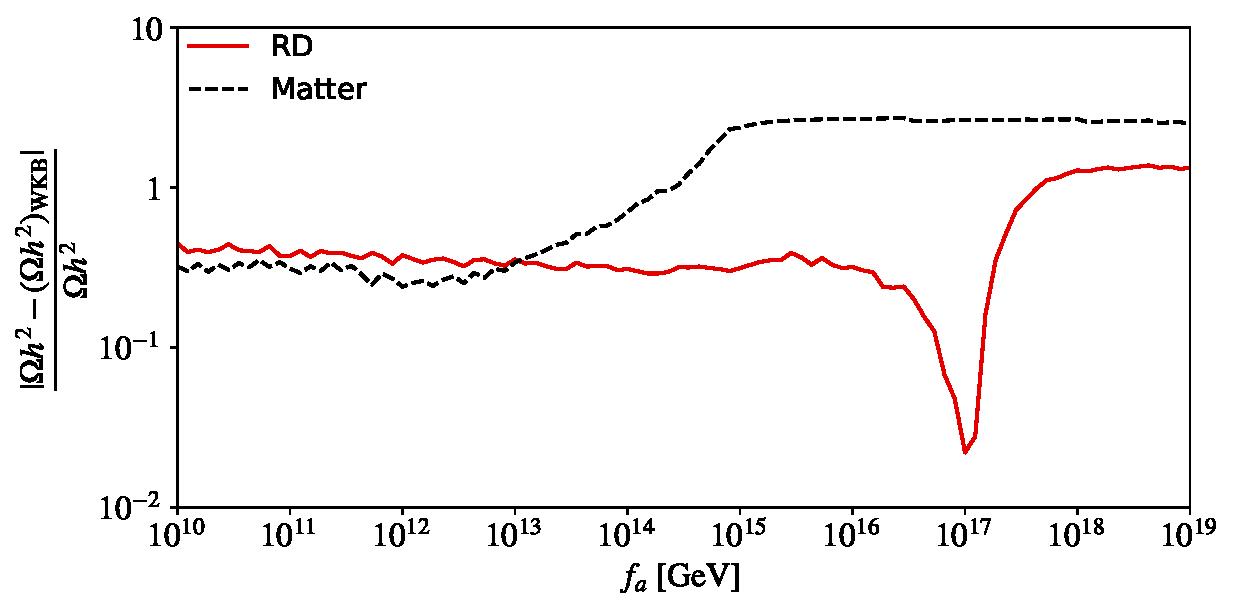
\includegraphics[width=1\textwidth]{figs/WKB_diff_i.pdf}
		\caption{}
		\label{fig:WKB_diff_i}
	\end{subfigure}
	\begin{subfigure}[]{0.5\textwidth}
		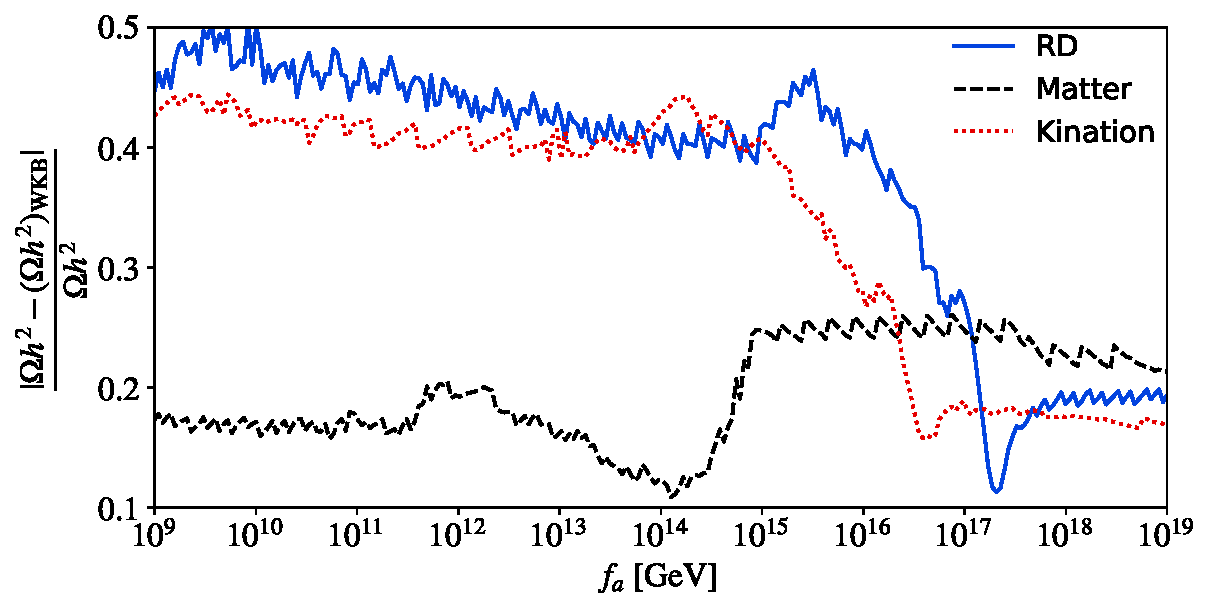
\includegraphics[width=1\textwidth]{figs/WKB_diff_osc.pdf}
		\caption{}
		\label{fig:WKB_diff_osc}
	\end{subfigure}
	\begin{center}
	\begin{subfigure}[]{0.5\textwidth}
		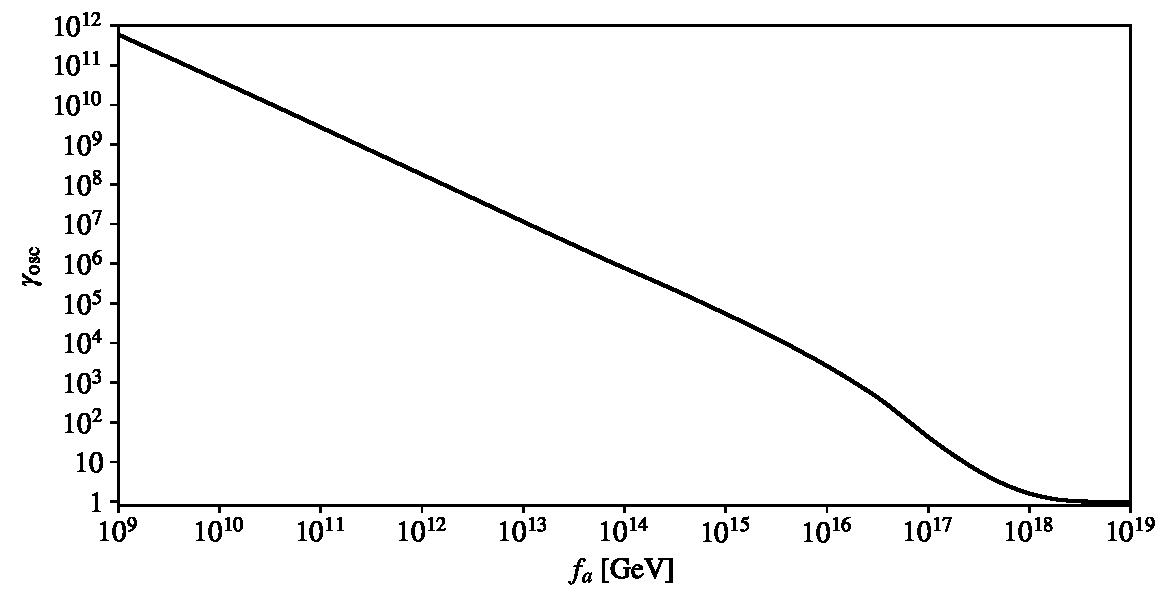
\includegraphics[width=1\textwidth]{figs/gamma_osc.pdf}
		\caption{}
		\label{fig:gamma_osc}
	\end{subfigure}
	\end{center}
\caption{...}
\label{fig:WKB_diff}
\end{figure}
%

Nevertheless, neither estimates based on \eqs{eq:solution_eom_approx_theta_osc,eq:solution_eom_approx_final} seem to provide a result comparable to numerically integrating \eqs{eq:eom_u}. Therefore, numerical integration should be preferred. 

\subsubsection{Adiabatic invariant and the anharmonic factor}\label{sec:an_fac}
%
In oscillatory systems with varying period, the energy is not conserved, and it is usually useful to define an ``adiabatic invariant", which is an approximate constant of motion.

\paragraph{Definition of the adiabatic invariant}
%
Given a system with Hamiltonian $\mathcal{H}(\theta,p;t)$, the equations of motion are 
%
\begin{equation}
	\dot p = - \dfrac{\partial \mathcal{H}}{\partial \theta} \;, \;\; 
	\dot \theta =  \dfrac{\partial \mathcal{H}}{\partial p} \;.
	\label{eq:hamiltonian_eoms}
\end{equation}

Moreover, we note that
%
\begin{equation}
	d \Ham = \dot \theta \ d p - \dot p \ d \theta + \dfrac{\partial \Ham}{\partial t} \ d t \;.  
	\label{eq:total_dH}
\end{equation}


If this system exhibits closed orbits (\eg if it oscillates), we define 
%
\begin{equation}
	J \equiv C \ \oint p \ d \theta \;,
	\label{eq:adiabatic_inv_def}
\end{equation}
%
where the integral is over a closed path (\eg a period, $T$), and $C$ indicates that $J$ can always be rescaled with a constant. This quantity is the adiabatic invariant of the system, if the Hamiltonian varies slowly during a cycle. That is,
%
\[
\dfrac{d J}{d t} = C \ \oint \lrBigb{\dot p \ d \theta + p \ d \dot \theta} = C \ \dint_{t}^{t+T}  \dfrac{\partial \Ham}{\partial t^\prime} \ d t^\prime \approx T \ \dfrac{\partial \Ham(t^{\prime})}{\partial t^{\prime}}\Big|_{t^{\prime}=t} \approx 0 
\;. 
\]
%




\paragraph{Application to the axion}
%
The Hamiltonian that results in the EOM of \eqs{eq:eom} is
%
\begin{equation}
	\Ham = \dfrac{1}{2} \dfrac{p^2}{\fa^2 \ a^3} + V(\theta) \ a^3\;,
	\label{eq:axion_H}
\end{equation}
%
with 
%
\begin{eqnarray}
	& p = \fa^2 \ a^3 \ \dot \theta \\
	\label{eq:momentum}
	& V(\theta) = \maT^2 \fa^2 (1-\cos \theta) \;.
	\label{eq:potential}
\end{eqnarray}

Notice that the Hamiltonian varies slowly if $\dot \maT/\maT \ll \maT$ and $H \ll \maT$, which are the adiabatic conditions.  When these conditions are met, the adiabatic invariant for this system becomes
%
\begin{equation}
	J = \dfrac{\oint p \ d \theta}{\pi \fa^2} = \dfrac{1}{\pi \fa^2} \oint \sqrt{ 2\lrb{ \Ham(\theta) - V(\theta) \ a^3} \ \fa^2 a^3 \ }  \ d \theta  =
	 \dfrac{2}{\pi \fa^2} \int_{-\thetamax}^{\thetamax} \sqrt{ 2\lrb{ \Ham(\thetamax) - V(\theta) \ a^3} \ \fa^2 a^3 \ } d \theta \;,
	 \label{eq:J_axion_definition}
\end{equation}
%
where we note that $\thetamax$ denotes the maximum of $\theta$ -- the peak of the oscillation, which corresponds to $p=0$. That is, $\Ham(\thetamax) = V(\thetamax) \ a^3$. Therefore, the adiabatic invariant, takes the form 

\begin{eqnarray}
	J=&  \dfrac{2 \sqrt{2} }{\pi \fa}  \int_{- \thetamax} ^{\thetamax}  \sqrt{ V(\theta_{\rm max}) - V(\theta) } a^{3} d \theta = 
	\dfrac{2 \sqrt{2} }{\pi} \ \maT \, a^3 \ \dint_{- \thetamax}^{\thetamax} \sqrt{\cos \theta - \cos \thetamax} \ d \theta  
	\;,
	\label{eq:J_axion_derivation}
\end{eqnarray}
%
where, for the last equality. we have used the adiabatic conditions, \ie negligible change of $\maT$ and $a$ during one period. Usually, the adiabatic invariant is written as~\cite{Lyth:1991ub,Bae:2008ue} 
%
\begin{equation}
	J = a^3 \ \maT \ \thetamax^2  \, f(\thetamax)  \;,
	\label{eq:J_axion_final_form}
\end{equation}
%
where 
\begin{equation}
	f(\thetamax) =\dfrac{ 2 \sqrt{2}}{\pi \thetamax^2 } \dint_{- \thetamax}^{\thetamax} d \theta \sqrt{ \cos \theta - \cos \thetamax } \;,
	\label{eq:anharmonic_f}
\end{equation}
%
is called the anharmonic factor, with $ 0.5 \lesssim f(\thetamax) \leq 1$ (see \Figs{fig:anharmonic_factor}).


\begin{figure}[t]
	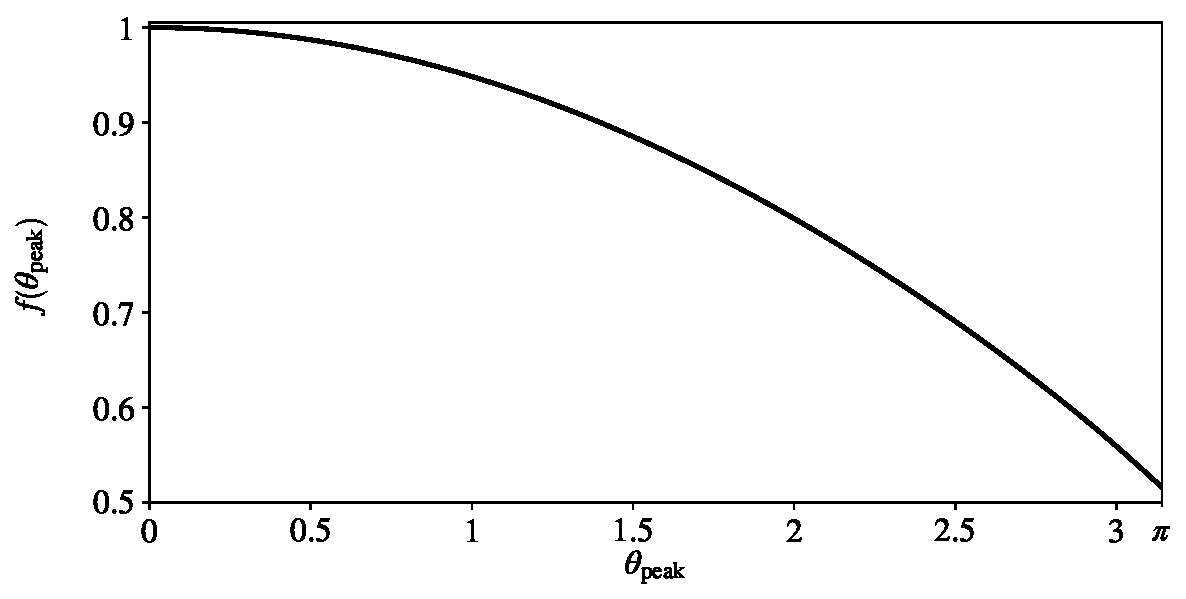
\includegraphics[width=1\textwidth]{figs/anharmonic_factor.pdf}
	\caption{The anharmonic factor for $0 \leq \thetamax < \pi $.}
	\label{fig:anharmonic_factor}
\end{figure}



\paragraph{The role of the adiabatic invariant in the axion relic energy density}
%
The adiabatic invariant allows us to calculate the maximum value of the angle $\theta$ at late times from its corresponding value at some point after the adiabatic conditions where met. It allows us to calculate the energy density of the axions field for $\theta \gtrsim 1$ since we have taken into account the exact potential.

In order to do this, we can numerically integrate \eqs{eq:eom}, and identify the maxima of $\theta$. Once the adiabatic conditions are fulfilled, we can stop the integration at a peak, $\thetamax_{,*}$ -- which corresponds to $T=T_{*}$ and $a=a_{*}$. Then, the value of the maximum angle today ($\thetamax_{,0} \ll 1$) is related to $\thetamax_{,*}$ via
%
\begin{eqnarray}
	\thetamax_{,0}^2 &=  \lrb{\dfrac{a_*}{a_0}}^3 \ \dfrac{\maT_{,*}}{\ma} \ f(\thetamax_{,*}) \ \thetamax_{,*}^2  =
	\gamma^{-1} \ \dfrac{s_0}{s_*} \ \dfrac{\maT_{,*}}{\ma} \ f(\thetamax_{,*}) \ \thetamax_{,*}^2 
	\; .
	\label{eq:theta_relation}
\end{eqnarray}
%
Using this, and since we evaluate the energy density at the maximum of $\theta$ (\ie $\dot \theta = 0$), we can determine the energy density of axions today from \eqs{eq:rho_a_def}. That is,
%
\begin{equation}
	\rho_{a,0} = \gamma^{-1} \ \dfrac{s_0}{s_*} \ \ma \ \maT_{,*} \ \dfrac{1}{2} \ \fa^2 \ \thetamax_{,*}^2 \;  \ f(\thetamax_{,*}) \;.
	\label{eq:rho_axion_exact}
\end{equation}
%
Notice that this is form of $\rho_{a,0}$  is similar to the the WKB result~(\ref{eq:rho_a_approx}) at $\tosc \to t_*$, multiplied by the anharmonic factor $f(\thetamax_{,*})$. That is, if the axion starts to evolve adiabatically close to $t=\tosc$, and $\thetaosc \ll 1$, the WKB approximation is valid.






\section{How to start using \mimes}\label{sec:start}
\setcounter{equation}{0}
%
\begin{listing}
	\begin{bash}
		git clone git@github.com:dkaramit/MiMeS.git
		cd MiMeS
		git submodule init
		git submodule update --remote
	\end{bash}
	%
	\caption{Commands in order to download \mimes, the differential equation solvers, and the interpolation libraries.}
	\label{list:git_download}
\end{listing}
%
The library can downloaded from \href{https:/github.com/dkaramit/MiMeS}{github.com/dkaramit/MiMeS}. Since the library depends on {\tt NaBBODES}~\cite{NaBBODES} {\tt SpleSplines}~\cite{SimpleSplines}, one has to download the, too. However, in order to get \mimes ready, one can run the commands shown in listing~\ref{list:git_download}. Although this method should be preferred in order to get the latest version, \mimes can also be downloaded from \href{https:/mimes.hepforge.org/downloads/}{mimes.hepforge.org/downloads}.


Once everything is downloaded successfully, we can go inside the \mimes directory, and run \run{bash configure.sh}~\footnote{It is recommended to use {\tt bash}.} and \run{make}.  The {\tt bash} script {\tt configure.sh}, just writes some paths to some files, formats the data files provided in a acceptable format (in section~\ref{sec:input} the format is explained), and makes some directories.
%
The {\tt makefile} is responsible for compiling some examples and checks, as well as the shared libraries that needed for the \PY interface.  If everything runs successfully, there should be two new directories {\tt exec} and {\tt lib}. Inside {\tt exec}, there are several executables that ready to run, in order to ensure that the code runs (\eg no segmentation fault occurs). For example, {\tt exec/AxionSolve\_check.run}, should print the values of the parameters $\thetai$ and $\fa$, the oscillation temperature and the corresponding value of $\theta$, the evolution of the axion (\eg temperature, $\theta$, $\rho_{a}$, etc.), and the values of various quantities on the peaks of the oscillation.  In the directory {\tt lib}, there are several shared libraries for the \PY interface.

\subsection{First steps}\label{sec:first_steps} 
%
There are several examples in \CPP ({\tt MiMeS/UserSpace/Cpp}) and \PY ({\tt MiMeS/UserSpace/Python}), as well as \JUPY  notebooks ({\tt MiMeS/UserSpace/JupyterNotebooks}), that show in detail how \mimes can be used. 

\subsubsection{Using \mimes in \CPP} 
%
In order to use the {\tt mimes::Axion<LD>} class in a \CPP program, we need ti include the header file {\tt AxionSolve.hpp} located in {\tt MiMeS/src/Axion}. That is, on top of the {\tt .cpp}, we need to write 
%
\begin{cpp}
	#include "MiMeS/src/Axion/AxionSolve.hpp"
\end{cpp}
%
Notice that if the  {\tt .cpp} is not in the root directory of \mimes, we need to compile it using the flag {\tt -Ipath-to-root}, "path-to-root" the relative path to the root directory of \mimes; \eg if the {\tt .cpp} is in the {\tt MiMeS/UserSpace/Cpp/Axion} directory, this flag should be {\tt -I../../../}.

Then, we can assign an instance of {\tt mimes::Axion<LD>} in a variable using
%
\begin{cpp}
	mimes::Axion<LD> ax(theta_i, fa, umax, TSTOP, ratio_ini, N_convergence_max,convergence_lim,
	inputFile, initial_step_size,minimum_step_size, maximum_step_size, absolute_tolerance, 
	relative_tolerance, beta, fac_max, fac_min, maximum_No_steps);
\end{cpp}
%
Here, {\tt LD} should be the desirable numeric type to be used; it is advised to use {\tt long double}, but other choices are also available as discussed later. The various parameters are as follows:
%
\begin{enumerate}
	\item {\tt theta\_i}: initial angle.
	\item {\tt fa}: the PQ scale.
	\item {\tt umax }: if $u>${\tt umax} the integration stops (remember that $u=\log(a/a_i)$). Typically, this should be a large number ($\sim 1000$), in order to avoid stopping the integration before the axion begins to evolve  adiabatically.    
	\item {\tt TSTOP}: if the temperature drops below this, integration stops. In most cases this should be around 
	$10^{-4}~\GeV$, in order to be sure that any entropy injection has stopped before integration stops (since BBN bounds~\cite{Kolb:206230,Peebles:1993} should not be violated).
	\item {\tt ratio\_ini}: integration starts when $3H/\maT \approx${\tt ratio\_ini} (the exact point depends on the file ``{\tt inputFile}", which we will see later). 
	\item  {\tt N\_convergence\_max} and {\tt convergence\_lim}: integration stops when the relative difference 
	between two consecutive peaks is less than {\tt convergence\_lim} for {\tt N\_convergence\_max} 
	consecutive peaks.
	\item  {\tt inputFile}: relative (or absolute) path to a file that describes the cosmology. the columns should be: $u$ $T ~[\GeV]$ $\log H$, sorted so that $u$ increases.~\footnote{One can run \run{bash MiMeS/src/FormatFile.sh inputFile} in order to sort it and remove any unwanted duplicates. See Appendix~\ref{app:util} for details of {\tt MiMeS/src/FormatFile.sh}.}
	%
	It is important to remember that \mimes assumes that the entropy injection has stopped before the lowest temperature of given in {\tt inputFile}. Since \mimes is unable to guess the cosmology beyond what is given in this file, the user has to make sure that there are data between the initial temperature (which corresponds to {\tt ratio\_ini}, and {\tt TSTOP}).
	
	\item {\tt initial\_stepsize} (optional): initial step the solver takes. 
	
	\item {\tt maximum\_stepsize} (optional): This limits the step-size to an upper limit. 
	\item {\tt minimum\_stepsize} (optional): This limits the step-size to a lower limit. 
	
	\item {\tt absolute\_tolerance} (optional): absolute tolerance of the RK solver
	
	\item {\tt relative\_tolerance} (optional): relative tolerance of the RK solver.
	%
	Generally, both absolute and relative tolerances should be $10^{-8}$. 
	In some cases, however, one may need more accurate result (\eg if {\tt f\_a} is extremely high, 
	the oscillations happen violently, and the system destabilizes). Whatever the case, if the  
	tolerances are below $10^{-8}$, long doubles have be used. \mimes by default uses {long double} variables, 
	in order to change it see the options available in section~\ref{sec:input}.
	
	\item {\tt beta} (optional): controls how agreesive the adaptation is. Generally, it should be around but less than 1.
	
	\item {\tt fac\_max},  {\tt fac\_min} (optional): the stepsize does not increase more than fac\_max, and less than fac\_min. 
	This ensures a better stability. Ideally, {\tt fac\_max}$=\infty$ and {\tt fac\_min}$=0$, but in reality one must 
	tweak them in order to avoid instabilities.
	
	\item {\tt maximum\_No\_steps} (optional): maximum steps the solver can take Quits if this number is reached even if integration
	is not finished. 
\end{enumerate}
%
in order to understand the usage of the optional parameters, some basic techniques of Runge-Kutta methods are discussed in Appendix~\ref{app:RK}. 

The EOM~(\ref{eq:eom_u}), then can be solved using 
%
\begin{cpp}
	ax.solveAxion();
\end{cpp}
%
This, if this runs successfully (in simple cases, such as a radiation dominated Universe, this should take a fraction of a second), then  $\Tosc$, $\thetaosc$, and $\Omega h^2$ are accessed via {\tt ax.T\_osc}, {\tt ax.theta\_osc}, and {\tt ax.relic}. The entire evolution (the points the integrator took) of the axion angle is stored in {\tt ax.points}, which is a two-dimensional {\tt std::vector}, with the columns corresponding to  $a$, $T~[\GeV]$, 
$\theta$, $d\theta/du$, $\rho_a$. Moreover, the peaks of he oscillation are stored in another two-dimensional {\tt std::vector}, with the columns corresponding to $a$, $T~[\GeV]$, $\thetamax$, $d\theta/du=0$, $\rho_a$, $J$. We should note that the peaks are identified using linear interpolation between integration points, in order to ensure that $d\theta/du = 0$. That is, the values stored in {\tt mimes::Axion<LD>::peaks} do not exist in {\tt mimes::Axion<LD>::points}.

The final member function is {\tt mimes::Axion<LD>::setTheta\_i}, which allows the user to set a different $\thetai$ without generating another instance.~\footnote{Since the interpolations of the data of {\tt inputFile} are made inside the constructor of the {\tt mimes::Axion<LD>} class, {\tt mimes::Axion<LD>::setTheta\_i} is a faster choice if ones needs to solve the EOM for a different initial condition.} This function is used as    
%
\begin{cpp}
	ax.setTeta_i(new_theta_ini);
\end{cpp}
%
where {\tt new\_theta\_ini} is the new value of $\thetai$. Running this function resets all variables to $0$ (except {\tt T\_osc} and {\tt a\_osc}, since they should not change), and clears all {\tt std::vector} variables, which allows the user to simply run \run{ax.solveAxion();} as if {\tt ax} was a freshly defined instance.  

\subsubsection{Using \mimes in \PY} The modules for the \PY interface are located in {\tt MiMeS/src/interfacePy}. Since, the most useful module is the one that actually solves the EOM~\ref{eq:eom_u}, we will explain here it can be used, and describe the others in Appendix~\ref{app:modules}.

The {\tt Axion} class in the module {\tt interfacePy.Axion} can be loaded in a \PY script as 
%
\begin{py}
	from sys import path as sysPath
	from os import path as osPath
	sysPath.append(osPath.join(osPath.dirname(__file__), 'path_to_src'))
	from interfacePy.Axion import Axion
\end{py}
%
It is important that \mintinline{python}{'path_to_src'} provides the relative path to the {\tt MiMeS/src} directory. For example, if the script is located in {\tt MiMeS/UserSpace/Python}, \mintinline{python}{'path_to_src'} should be \mintinline{python}{'../../src'}.

Once the module is imported, we can define an {\tt Axion} instance as follows 
%
\begin{py}
	ax=Axion(theta_i, fa, umax, TSTOP, ratio_ini, N_convergence_max, convergence_lim, inputFile,
	initial_step_size,minimum_step_size, maximum_step_size, absolute_tolerance, 
	relative_tolerance, beta, fac_max, fac_min, maximum_No_steps)
\end{py}
%
Here, {\tt Axion} is the constructor of the {\tt Axion} class, and {\tt ax} the variable -- which can have any name, and the input parameters are exactly the same as in the \CPP case (the usage of the class can be found by running {\tt ?Axion} after loading the module). 

Using the defined variable ({\tt ax} in this example), we can simply run  
%
\begin{py}
	ax.solveAxion()
\end{py}
%
in order to solve the EOM of the axion. In contrast to the \CPP implementation, this only gives us access to $\Tosc$, $\thetaosc$, and $\Omega h^2$; the corresponding variables are {\tt ax.T\_osc}, {\tt ax.theta\_osc}, and {\tt ax.relic}. In order to get the evolution of the axion field, we need to run 
%
\begin{py}
	ax.getPoints()
\end{py}
%
This will make {\tt numpy} arrays that contain the scale factor ({\tt ax.a}), temperature ({\tt ax.T}), $\theta$ ({\tt ax.theta}), its derivative with respect to $u$ ({\tt ax.zeta}), and the energy density of the axion ({\tt ax.rho\_axion}).

Moreover, in order to get the various quantities on the peaks of the oscillation, we can run
%
\begin{py}
	ax.getPeaks()
\end{py}
%
This makes {\tt numpy} arrays that contain the scale factor ({\tt ax.a\_peak}), temperature ({\tt ax.T\_peak}), $\theta$ ({\tt ax.theta\_peak}), its derivative with respect to $u$ ({\tt ax.zeta\_peak}, which should be equal to $0$), the energy density of the axion ({\tt ax.rho\_axion\_peak}), and the values of the adiabatic invariant on the peaks ({\tt ax.adiabatic\_invariant}).

The initial condition $\thetai$ can be changed using 
%
\begin{py}
	ax.setTeta_i(new_theta_ini)
\end{py}
%
which is faster than running the constructor again, since all the interpolations are reused. However, running this function, erases all the arrays, and resets all variables to $0$ (except {\tt T\_osc} and {\tt a\_osc}, as they should not change). 

\paragraph{Importand} Th {\tt Axion} class constructs a {\tt mimes::Axion<LD>} pointer, which has to be manually deleted. Therefore, once {\tt ax} is used it must be deleted, \ie we need to run 
%
\begin{py}
	del ax
\end{py}
%
We should note that this must run even if we assign another instance to the same variable {\tt ax}, otherwise we risk running out of memory.

\section{Assumptions and user input}\label{sec:assumptions}
\setcounter{equation}{0}
%
\mimes only makes a few, fairly general, assumptions. First of all, it is assumed that the axion energy density is always subdominant compared to radiation or any other component of the Universe, and that decays and annihilations of particles have a negligible effect on the axion energy density. Moreover, the initial condition is always assumed to be $\theta_{t=\ti} = \thetai$ and $\dot \theta|_{t=\ti}=0$. 
%
Furthermore, it is also assumed that $3H/\maT$ increases monotonically at high temperatures. 
%
Also, it is assumed that the entropy is resumes its conserved status at a temperature higher than the minimum temperature of  {\tt inputFile} (which is required by the constructor of the {\tt mimes::Axion<LD>} class).  
%
Finally, \mimes does not try to predict anything regarding the cosmology. Therefore, the temperatures in {\tt inputFile} {\em must} cover the entire region of  integration; \ie the maximum temperature has to be larger than the one required to reach {\tt ratio\_ini}, while the minimum one should be lower than {\tt TSTOP}.

\subsection{Options at Compile-time}
%
The user has a number of options regarding different aspects for the code. The various choices for the shared libraries used by the \PY interface are given in {\tt \mimes/Definitions.mk}. while the corresponding options for the \CPP examples are in the {\tt Definitions.mk} files in the directories inside {\tt \mimes/UserSpace/Cpp}.  The options correspond to different variables, which are
%
\begin{enumerate}
	\item {\tt rootDir}: the relative path of root directory of \mimes.  
	%
	\item {\tt LONG}: this should be either {\tt long} or omitted. If omitted, the type of the numeric values is {\tt double} (double precision). On the other hand, if {\tt LONG=long},  the type is  {\tt long double}. Generally, using {\tt double} should enough. For the sake of numerical stability, then, it is advised to always use {\tt LONG=long}, as it a safer option. The reason is that the axion angle redshifts, and can become very small, which introduces ``rounding errors". Moreover, if the parameters {\tt absolute\_tolerance} or {\tt absolute\_tolerance} are chosen to be below $\sim 10^{-8}$, then double precision numbers may not be enough, and {\tt LONG=long} is preferable.  This choice comes at the cost of speed; double precision operations are usually preformed much faster. It is important to note that {\tt LONG} defines a macro with the same name, which then defines the macro {\tt LD} (in all the {\tt .cpp} files) as {\tt \#define LD LONG double}.
	%
	\item {\tt LONGpy}: the same as {\tt LONG}, but for the \PY interface.
	%
	\item {\tt Solver}: \mimes uses the ordinary differential equation (ODE) integrators of ref.~\cite{NaBBODES}. Currently, there are two available choices; {\tt Rosenbrock} and {\tt RKF}. The former is a general embedded Rosenbrock implementation and it is used if {\tt Solver=1}, while the latter is a general explicit embedded Runge-Kutta implementation and can be chose by using {\tt Solver=2} (a brief description of how these algorithms are implemented can be found in Appendix~\ref{app:RK}). The default option for that \mimes uses is {\tt Solver=1}, because the axion EOM tends to oscillate rapidly. However, in some cases, a high order explicit method may also work. This variable, is used to define a macro with the same name and value in {\tt \mimes/src/Axion/AxionSolve.hpp}.
	%
	\item {\tt METHOD}: Depending on the type of solver is chosen, there are some available methods. 
		\begin{itemize}
			\item 	For {\tt Solver=1}, the available methods are 
			{\tt METHOD=RODASPR2} and {\tt METHOD=ROS34PW2}. The {\tt RODASPR2} choice is a fourth order Rosenbrock-Wanner method (more information can be found in ref.~\cite{RANG2015128}). The {ROS34PW2} choice corresponds to a third order Rosenbrock-Wanner method~\cite{RangAngermann2005}. 
			%
			\item 	For {\tt Solver=2}, the only reliable method available in {\tt NaBBODES} is the Dormand-Prince~\cite{DORMAND198019} chosen if {\tt METHOD=DormandPrince}, which is an explicit Runge-Kutta method of seventh order.
		\end{itemize}
		%
		It is worth mentioning that {\tt NaBBODES} is built in order to be a template for all possible Rosenbrock and explicit Runge-Kutta embedded methods, and one can provide their own Butcher tableau if they want to use another method, as shown in Appendix~\ref{app:RK}. This variable, is used to define a macro with the same name and value in {\tt \mimes/src/Axion/AxionSolve.hpp}.
	%
	\item {\tt CC}: the \CPP compiler that one chooses to use. The default option is {\tt CC=g++}, which is the {\tt GNU} \CPP compiler, and is available for all systems. Another option is to use the {\tt clang} compiler, which is chosen by {\tt CC=clang -lstdc++}. \mimes is mostly tested using {\tt g++}, but {\tt clang} also seems to work (and the resulting executables are sometimes faster), but the user has to make sure that their version of the compiler of choice supports the \CPP17 standard, otherwise \mimes probably will not work.
	%
	\item {\tt OPT}: Optimization level of the compiler. By default, this is {\tt OPT=O3}, which produces executables that are marginally faster than {\tt OPT=O1} and {\tt OPT=O2}, but significantly faster than {\tt OPT=O0}. There is another choice, {\tt OPT=Ofast}, but it can cause various numerical instabilities, and is generally considered dangerous -- although we have not observed any problems when running \mimes. 
\end{enumerate}
%
These options can only be used when the compilation is done using the various {\tt makefile} files. For manual compilation of a user provided {\tt .cpp} file, the options {\tt LONG}, {\tt Solver}, and {\tt METHOD} correspond to macros with the same name.~\footnote{Macros can be defined using the {\tt -D} flag
in the compiler. For example {\tt METHOD=DormandPrince} is the same as passing {\tt -DMETHOD=DormandPrince} to the compiler.} It should be pointed-out that {\tt LONG} is in the examples is used to define a macro {\tt LD} which becomes {\tt double} or {\tt long double} accordingly. the actual choice of numeric type is passed as a template parameter in all classes. Therefore, this macro alone does not automatically mean that the code is compiled using {\tt long double} numbers. In order to understand the template arguments of the classes, see section~\ref{sec:complete_examples}. 

\subsection{User input}\label{sec:input}
%
\subsubsection{Compile-time input}\label{sec:compile_time_input} 
%
\paragraph{Files} \mimes requires files that provide data for the relativistic degrees of freedom (RDOF) of the plasma, as well as its mass as a function of the temperature. Although \mimes is shipped with the standard model RDOF found in~\cite{Saikawa:2020swg}, and the axion mass from~\cite{Borsanyi:2016ksw}, the user can change the corresponding variables in {\tt Paths.mk} (found in the root directory of \mimes) to another file path. The variables pointing to these data files are {\tt cosmoDat} and {\tt axMDat}, for the RDOF and axion mass, respectively.~\footnote{One can change the data file for anharmonic factor introduced in \eqs{eq:anharmonic_f} using the variable {\tt anFDat}.}

The format of the files is the following:~\footnote{The anharmonic factor data are given in $\thetamax$ $f(\thetamax)$, with increasing $\thetamax$.} 
%
\begin{itemize}
	\item The RDOF data must be given in three columns; $T$ (in $\GeV$), $\heff$, and $\geff$.
	%
	\item The axion mass data must be given in two columns; $T$ (in $\GeV$), $\chi$ (in $\GeV^4$). Here, $\chi$ is defined as in \eqs{eq:axion_mass_def}. 
	The user can provide a function instead of data for the axion mass, by leaving the  {\tt axMDat} variable empty. 
\end{itemize}
%
The paths to these files should be given at compile time. That is, once {\tt Paths.mk} changes, \run{bash configure.sh} and then \run{\tt make} must be ran. The user can change the content of the data files (without changing their paths), in order to use them without compiling \mimes again. However, the user has to make sure that all the files are sorted so that the values of first column increase (with no duplicates or empty lines). In order to ensure this, it is advised to run \run{bash FormatFile.sh path-to-file} (in Appendix~\ref{app:util} there are some details on {\tt MiMeS/src/FormatFile.sh}), in order to format the file (that should exist in \run{path-to-file}) complies with the requirements of \mimes.

\paragraph{Static variables} The header file {\tt MiMeS/src/static.hpp} contains definitions of various static variables that are used in the \PY modules and the {\tt mimes::Axion<LD>} class. These variables are instances of  {\tt mimes::Cosmo<LD>}, {\tt mimes::AxionMass<LD>}, and {\tt mimes::AnharmonicFactor<LD>}, and they are responsible for interpolation of the various plasma parameters (\ie $\heff(T)$, $\geff(T)$, $s(T)$, etc.), the axion mass, and the anharmonic factor, respectively.

\subparagraph{{\tt cosmo<LD>}} The static variable {\tt cosmo<LD>} is an instance of {\tt mimes::Cosmo<LD>}, with {\tt LD} being a numeric type (\eg {\tt double}, {\tt long double}). It is expected to be defined in {\tt MiMeS/src/static.hpp}, as 
%
\begin{cpp}
	template<class LD> static mimes::Cosmo<LD> cosmo(cosmo_PATH,minT,maxT);
\end{cpp}
%
The arguments of the constructor are
%
\begin{enumerate}
	\item {\tt cosmo\_PATH}: a string of the absolute path of the relativistic degrees of freedom (RDOF). This macro is automatically
	written in {\tt MiMeS/src/misc\_dir/path.hpp} when \run{bash configure.sh} is ran. The RDOF data must be given in three columns; $T$ (in $\GeV$), $\heff$, and $\geff$.
	%
	\item {\tt minT} (optional): The minimum interpolation temperature. Bellow this limit, $\heff$ and $\geff$ are takes to be constant. Its default value is $0$.
	%
	\item {\tt maxT} (optional): The maximum interpolation temperature. Above this limit, $\heff$ and $\geff$ are takes to be constant. Its default value is $m_P$; the Planck mass $m_P = 1.22 \times 10^{19}~\GeV$.
\end{enumerate} 
%
It should be noted that  the interpolation limits {\tt minT} and {\tt maxT} are suggestions; the actual limits will be set to their closest value that exist in the data file. Apart form the various member functions, there are several static variables; \eg the CMB temperature today ({\tt mimes::Cosmo<LD>::T0}), the Planck mass ({\tt mimes::Cosmo<LD>::mP}), etc. The values of all these parameters are taken as compile-time constants. However, the user can change their values directly from the class, which is located in {\tt \mimes/src/Cosmo/Cosmo.hpp}.


\subparagraph{{\tt axionMass<LD>}} The static  variable {\tt axionMass<LD>} is an instance of {\tt mimes::AxionMass<LD>}. It is expected to be defined in  {\tt MiMeS/src/static.hpp}. The first way one can define the variable {\tt axionMass<LD>} is
%
\begin{cpp}
	template<class LD> static mimes::AxionMass<LD> axionMass(chi_PATH,minT,maxT);
\end{cpp}
%
The arguments of the constructor are
%
\begin{enumerate}
	\item {\tt chi\_PATH}: a string of the absolute path of the data for $\chi$ (defined as in \eqs{eq:axion_mass_def}). This macro is automatically
	written in {\tt MiMeS/src/misc\_dir/path.hpp} when \run{bash configure.sh} is ran. The data must be given in two columns; $T$ (in $\GeV$), $\chi$ (in $\GeV^4$).
	%
	\item {\tt minT} (optional): The minimum interpolation temperature. Its default value is $0$.
	%
	\item {\tt maxT} (optional): The maximum interpolation temperature.Its default value is $m_P$.
\end{enumerate} 
%
As previously, the interpolation limits {\tt minT} and {\tt maxT} are suggestions, as the actual limits will be set to the closest value that exist in the data file. Beyond these limits, the axion mass by default is taken to be 
%
\begin{equation}
	\maT = \Bigg\{
	\begin{matrix}
		\dfrac{\chi(T_{\rm min})}{\fa^2} & \text{for } T<T_{\rm min} 
		\\ \\
		\dfrac{\chi(T_{\rm max})}{\fa^2}   \lrb{\dfrac{T}{T_{\rm max}}}^{-8.16} & \text{for } T>T_{\rm max} 
	\end{matrix} \;.
\end{equation}
%
This is a good approximation for the QCD axion (the default data \mimes uses), but the user can change them inside the class, which is located in{\tt \mimes/src/AxionMass/AxionMass.hpp} (see Appendix~\ref{app:classes} for details). 


The second way we can declare the {\tt axionMass<LD>} variable is
%
\begin{cpp}
	template<class LD> static mimes::AxionMass<LD> axionMass(ma2);
\end{cpp}
%
where {\tt ma2} -- the axion mass squared in $\GeV^2$ -- is a function object with signature {\tt LD ma2 (LD T, LD fa)}. In order to do this, 
the user may omit a data file path for the {\tt axMDat} variable in {\tt \mimes/src/Definition.mk}.

\subparagraph{{\tt anharmonicFactor<LD>}} The static variable {\tt anharmonicFactor<LD>} is an instance of the class {\tt mimes::AnharmonicFactor<LD>}. It is expected to be defined in  {\tt MiMeS/src/static.hpp}, as 
%
\begin{cpp}
	template<class LD> static mimes::AnharmonicFactor<LD> anharmonicFactor(anF_PATH);
\end{cpp}
%
Here,~{\tt anF\_PATH} is a macro of a string of the absolute path of the data for the anharmonic factor. This macro is automatically
written in {\tt MiMeS/src/misc\_dir/path.hpp} when \run{bash configure.sh} is ran. The data should be given in two columns; $\thetamax$, $f(\thetamax)$.

\subsubsection{Run-time input}\label{sec:run_time_input}
%
The run-time user input is described in sec.~\ref{sec:first_steps}. The user has to provide at least the parameters that describe the axion evolution, $\thetai$ and $\fa$. 

Moreover,  the maximum allowed value of $u$ and the minimum value of $T$, allow the user to decide when the integration has to stop even if the axion has not reached its adiabatic evolution. Ideally, {\tt umax}$=\infty$ and {\tt TSTOP}$=0$, but \mimes is designed to be as general as possible and there may be cases where one needs to stop the integration abruptly.~\footnote{These two variables are not optional, because the user must be aware of them, in order to choose them according to their needs.}

Furthermore, {\tt ratio\_ini} allows the user to choose a desired point at which the interpolation of the data in {\tt inputFile} begins. This can save valuable computation time as well as memory, as only the necessary data are stored and searched. Generally, for {\tt ratio\_ini}$>10^{3}$, the relic abundance becomes
independent from  {\tt ratio\_ini}, but one has to choose it carefully, in order to find a balance between accuracy and computation time.

Finally, the convergence conditions -- \ie~{\tt N\_convergence\_max} and {\tt convergence\_lim} -- allow the user to decide when the adiabatic evolution of the axion begins. Generally, the relic abundance does not have a strong dependence on these parameters as log as they are  {\tt N\_convergence\_max}$>3$ and {\tt convergence\_lim}$<10^{-1}$ (\ie the adiabatic invariant does not vary more that $10\%$ for three consecutive peaks of the oscillation). 
%
However, we should note that greedy choices (\eg~{\tt N\_convergence\_max}$=100$ and {\tt convergence\_lim}$=10^{-5}$) are dangerous, as $\theta$ tends to oscillate rapidly and destabilize the differential equation solver. Therefore, these parameters should be chosen carefully, in order to ensure that integration stops when axion has reached its adiabatic evolution, without destabilising the EOM.



\subsection{Complete Examples}\label{sec:complete_examples}

\paragraph{A complete \CPP example}\DK{Give the code with explanation of {\tt MiMeS/UserSpace/CPP/Axion}, along with the compilation options, and explain the template arguments.}

\paragraph{A complete \PY example}\DK{Give th/e code with explanation of {\tt MiMeS/UserSpace/Python/Axion.py}, say that the compilation options are set in the root directory of \mimes.}

\DK{Mention optimization options, and {\tt g++} and {\tt clang} seem to work. Describe the available solvers (appendix for more details).}.


	%%%%%%%%%%%%%%%%%%%%%%%%%%%%%%%%%%%%%%%%
% APPENDICES
%\pagebreak
%%%%%%%%%%%%%%%%%%%%%%%%%%%%%%%%%%%%%%%%
\setcounter{section}{0}
\section*{Appendix}
\appendix

\renewcommand{\theequation}{\Alph{section}.\arabic{equation}}
\setcounter{equation}{0}  % reset counter
%%%%%%%%%%%%%%%%%%%%%%%

\section{Basics of embedded Runge-Kutta Mehtods}\label{app:RK}
\setcounter{equation}{0}
%
Runge-Kutta (RK) methods are employed in order to solve an ordinary differential equation (ODE), or a system of ODEs of first order.~\footnote{Boundary value problems, and higher order differential equations are expressed as first order ODEs, and then solved.}   Although there are some very insightful sources in the literature (\eg~\cite{Hairer,hairer2010solving,10.5555/1403886}) we give a brief overview of them in order to help the user to make appropriate decisions when using \mimes.

The general form of a system of first order of ODEs is
%
\begin{equation}
	\dfrac{d\vec{y}}{dt}=\vec{f}(\vec{y},t) \;,
	\label{eq:ODE_definition}
\end{equation}
%
with given initial condition $\vec{y}(0)$. Also, the components of $\vec{y}$ denote the unknown functions. Note that we can always shift $t$ to start at $0$, which simplifies the notation. In order to solve the the system of \eqs{eq:ODE_definition}, an RK method uses an iteration of the form 
%
\begin{equation}
	\vec{y}_{n+1}=\vec{y}_{n}+ h\sum_{i=1}^{s} b_i \ \vec{k}_i \;,
	\label{eq:RK_iter}
\end{equation}
%
with $n$ denoting the iteration number, $h$ the ``step-size" that is used to progress $t$; $t_{n+1}=t_{n}+h$. Moreover, $s$, $b_i$ and $\vec{k}_i$ define the corresponding RK method. For example,
the classic Euler method is an RK method with $s=1$, $b=1$, and $\vec{k}_1 = \vec{f}(\vec{y_n , t_n})$. Methods with $\vec{k}$ that depends on previous step (\ie $\vec{k} =\vec{k}\lrsb{y_{n},t_{n}}$), are called explicit, while the ones that try to also predict next step (\ie $\vec{k} =\vec{k}\lrsb{y_{n},t_{n}; y_{n+1},t_{n+1}}$) are called implicit. 

\subsection{Embedded RK methods}
%
A large category of RK methods are  the so-called embedded RK methods. These methods make two estimates for the same step simultaneously -- without evaluating  $\vec{k}$ many times within the same iteration. Therefore, together with the iteration of \eqs{eq:RK_iter}, a second estimate is given by
%
\begin{equation}
	\vec{y}_{n+1}^{(*)}=\vec{y}_{n}+ h\sum_{i=1}^{s} b_i^{(*)} \vec{k}_i \;,
	\label{eq:RK_Embedded_iter}
\end{equation}
%
with $b_i^{(*)}$ is an extra parameter that characterise the ``embedded" method of different order (typically, one order higher that the estimate~\ref{eq:RK_iter}). The local (for the step $t_{n+1}$) error is, then, estimated as
%
\begin{equation}
	\epsilon \equiv  \sqrt{\frac{1}{N}\sum_{d=1}^{N}\lrb{\frac{y_{n+1 ,d}-y^{*}_{n+1,d}}{ \Lambda_d }}^{2}} \;,
	\label{eq:error_estimate}
\end{equation}
%
where $n$ the iteration number, $N$ the number of ODEs, $d$ the component of $\vec{y}$, and $\Lambda_d$ defined as 
%
\begin{equation}
	\Lambda_d = {\tt Atol} + \max\lrb{|y_{n+1, d}|,|y^{*}_{n+1 ,d}|} \; {\tt Rtol} \;,
	\label{eq:RK_scale}
\end{equation}
%
with {\tt Atol} and {\tt Rtol} the absolute and relative tolerances that characterise the desirable accuracy we want to achieve; user defined values, typically {\tt Atol}$=${\tt Rtol}$\ll 1$.  With these definitions, the desirable error is reached when  $\epsilon \lesssim 1$. 

\paragraph{Step-control} The definition~\ref{eq:error_estimate}, allows us to adjust the step-size $h$ in such way that $\epsilon \approx 1$. That is, we take trial steps, and $h$ is adapted until $\epsilon \approx 1$.  A simple adaptive strategy adjusts step-size, using
%
\begin{eqnarray}
	h \to \beta \; h \;  {\rm max} \lrsb{f_{\rm min}, {\rm min} \lrb{\epsilon^{-\frac{1}{p+1}}, f_{\rm max}}} \;,
	\label{eq:step-control}
\end{eqnarray}
%
with $p$ the order of the RK method ($p+1$ is the order of the embedded one), $\beta$  a bias factor of the adaptive strategy (typically $\beta$ is close but below $1$), used to adjust the tendency of $h$ to be somewhat smaller than what the step-control predicts. Also, $f_{min}$ and $f_{max}$ are the minimum and maximum allowed factors, respectively, that can multiply $\beta \ h$, used in order to avoid large fluctuations that can destabilise the process. All these parameters are chosen by the user, in order to make the step-control process as aggressive or safe as needed. 

\paragraph{Correspondence between \mimes parameters and RK ones}
%
The various parameters that \mimes are described in section~\ref{sec:input}. The correspondence between them and the RK parameters is given in table~\ref{tab:RK_mimes_params}.
%
\begin{table}[t!]
	\centering
	\begin{tabular}{|c|c|}
		\mimes & Runge-Kutta \\
		\hline
		{\tt absolute\_tolerance } & {\tt Atol}  \\
		\hline
		{\tt relative\_tolerance } & {\tt Rtol}  \\
		\hline
		{\tt b} & $\beta$  \\
		\hline
		{\tt fac\_min} & $f_{\rm min}$  \\
		\hline
		{\tt fac\_max} & $f_{\rm max}$  \\
		\hline
	\end{tabular}
	\caption{Correspondence between the user \mimes user input and the RK parameters described in the text.}
	\label{tab:RK_mimes_params}
\end{table}

\subsection{Explicit embedded RK methods}
%
Explicit methods use only the information of the previous step in order to compute $\vec{k}_i$ from  
%
\begin{equation}
	\vec{k}_{i}=\vec f\lrBiggb{ \vec{y}_{n}+h \lrBigb{ \sum_{j=1}^{i-1}a_{ij}\vec{k}_{j} }, t_{n}+ c_{i} \; h}\;, \quad \forall i=1,2,\dots, s\;,
	\label{eq:explicit_RK_k}
\end{equation}
%
with $a_{ij}$, $c_i$, together with $b_i$ and $b_i^{(*)}$, consist the so-called Butcher tableau of teh corresponding method. For explicit methods this is usually presented as 
%
\begin{equation}
	\begin{array}{c|cccccc}
		0      & 0      &   0   &      0& \dots & 0& 0\\
		c_2    & a_{21} &   0   &   0   & \dots & 0& 0\\
		c_3    & a_{31} & a_{32}&      0& \dots & 0& 0\\
		\vdots & \vdots & \vdots& \vdots&\ddots &\ddots& \vdots\\
		c_s    & a_{s1} & a_{s2}& a_{s3}& \dots & a_{s s-1}& 0 \\
		\hline
		p      & b_1    & b_2  & b_3 & \dots & b_{s-1} & b_s \\
		p+1      & b_1^{\star}    & b_2^{\star}  & b_3^{\star} & \dots & b_{s-1}^{\star} & b_s^{\star}
	\end{array}
	\label{eq:Butcher}
\end{equation}
%
It should be noted that $c_i = \displaystyle\sum_{j=1}^{s} a_{ij} $.

\subsection{Rosenbrock methods}
%
Explicit RK methods, encounter instabilities when a system is ``stiff"~\footnote{A definition of stiffness can be found in~\cite{hairer2010solving,Hairer}.}; when is oscillates rapidly, or has different elements at different scales. This problems are somewhat resolved by trying to predict the next step inside $\vec{k}$; \ie in implicit methods. However, then one has to solve a non-linear set of equations in order to compute $\vec{y}_{n+1}$, which is generally a slow process, as the Newton method (or some variation) needs to be applied. However, there exist another way, a compromise between explicit and implicit methods.  Linearly implicit RK methods, usually called Rosenbrock methods -- with popular improvements as Rosenbrock-Wanner methods, introduce  parameters in the diagonal of the Butcher tableau~\ref{eq:Butcher} and linearise the system of  non-linear equations (for details, see~\cite{hairer2010solving}). In these methods, $\vec{k}$ is determined by  
%
\begin{equation}
	\left(\hat I - \gamma h \hat{J}\right)\cdot \vec{k}_{i}=
	h \vec{f}\Big(\vec{y}_n+\sum_{j=1}^{i-1}a_{ij}\vec{k}_{j},t_n + c_{i}h \Big)+
	h^2 \left(\gamma + \sum_{j=1}^{i-1}\gamma_{ij}\right)\dfrac{\partial \vec{f} }{\partial t}+
	h \hat J \cdot \sum_{j=1}^{i-1}\gamma_{ij} \vec{k}_{j}\; ,
	\label{eq:Ros_k}
\end{equation}
%
which is written in such a way that everything is evaluated at $t = t_{n}$. In \eqs{eq:Ros_k},  $\hat J = \dfrac{\partial \vec f}{ \partial \vec y}$ the Jacobian of the system of ODEs, $\hat I$ the unit matrix with dimension equal to the number of ODEs. Moreover, $\gamma$ and $\gamma_{ij}$ are parameters that characterise the method (along with $a_{ij}$, $c_i$,  $b_i$, and $b_i^{(*)}$).

\paragraph{Implementing a new Butcher tableau in {\tt NaBBODES}} As already mentioned, \mimes uses {\tt NaBBODES}, which supports the implementation of new Butcher tableaux. This is done by adding a new class (or struct) inside the header file {\tt METHOD.hpp} that can be found in {\tt \mimes/src/NaBBODES/RKF} for the explicit RK and  {\tt \mimes/src/NaBBODES/Rosenbrock} for the Rosenbrock embedded methods. All the new parameters must be {\tt public},  {\tt constexpr static} variables, of a type that is the template parameter of the method. For example, the Heun-Euler method can be implemented, adding the following code in  {\tt \mimes/src/NaBBODES/RKF/METHOD.hpp}
%
\begin{cpp}
	/*-----Implementation of the Heun-Euler method-----*/
	/*-----It shouldn't be used for MiMeS, since it is likely to fail-----*/
	
	//LD is the numeric type (\ie double, or long double).
	template<class LD>
	//use struct because its variables are public by default.
	struct HeunEuler{  
		static constexpr unsigned int s=2; // HeunEuler is a 2-stage RK
		static constexpr unsigned int p=1; // order is 1 (its embedded order is p+1=2)

		//these are aliases for the arrays
		using arr=std::array<LD,s>;
		using arr2=std::array<std::array<LD,s>,s>;
		
		static constexpr arr b={0.5,0.5}; // this is $b_i$
		static constexpr arr bstar={0.5,0.5}; // this is $b_i^{(*)}$
		static constexpr arr c={0,1}; // remember that $c_i = \displaystyle\sum_{j=1}^{s} a_{ij}$
		
		// this is $a_{ij}$
		static constexpr arr2 a={
			arr{0,0},
			arr{1,0}
		};			
	};
\end{cpp}

In order to implement the ROS3w~\cite{RangAngermann2005} method, one can add the following code in the header file {\tt \mimes/src/NaBBODES/Rosenbrock/METHOD.hpp}
%
\begin{cpp}
	/*-----Implementation of the ROS3w method-----*/
	/*-----It shouldn't be used for MiMeS, since it is likely to fail-----*/
	
	
	//LD is the numeric type (\ie double, or long double).
	template<class LD>
	struct ROS3w{
		static constexpr unsigned int s=3; // 3-stage
		static constexpr unsigned int p=2; // second order (embedded order is $p+1$)
		
		//aliases for the arrays
		using arr=std::array<LD,s>;
		using arr2=std::array<std::array<LD,s>,s>;

		static constexpr arr b={0.25,0.25,0.5 };  // this is $b_i$
		// this is $b_i^{(*)}$
		static constexpr arr bstar={ 0.746704703274,0.1144064078371,0.1388888888888};  
		
		static constexpr arr c={0,2/3.,4/3.}; // remember that $c_i = \displaystyle\sum_{j=1}^{s} a_{ij}$
		static constexpr LD gamma=0.4358665215084; // this is $\gamma$
		
		// this is $a_{ij}$
		static constexpr arr2 a={
			arr{0,0,0},
			arr{2/3.,0,0},
			arr{2/3.,2/3.,0}	
		};
	
		// this is $\gamma_{ij}$	
		static constexpr arr2 g={
			arr{0,0,0},
			arr{0.3635068368900,0,0},
			arr{-0.8996866791992,-0.1537997822626,0}
		};
	};
\end{cpp}

\paragraph{How to compile \mimes in order to use the newly implemented method} One a new Butcher tableau is implemented, the {\tt mimes::Axion} class can use it. This class, needs the name of method assigned to the macro {\tt METHOD}. That is, before you include the header file {\tt src/Axion/AxionSolve.hpp}, this macro needs to be defined. A convenient way to do this, is to define the macro using the {\tt -D} flag of the compiler; \eg in order to use the ROS3w method, this definition ca be done by adding  {\tt -DMETHOD=ROS3w} when compiling the code. Alternatively, if one uses the {\tt makefile} files, a method can be chosen by adding it in the corresponding {\tt Definitions.mk} file as {\tt METHOD=ROS3w}.~\footnote{One make sure to use the correct {\tt Solver} macro -- {\tt Solver=1} for Rosenbrock method  and {\tt Solver=2} for explicit RK method-- otherwise the compilation will fail.} 


\section{\CPP classes}\label{app:classes}
\setcounter{equation}{0}
\DK{Describe all the classes.}

\section{\PY modules}\label{app:modules}
\setcounter{equation}{0}
\DK{Describe the modules.}



\section{Utilities}\label{app:util}
\setcounter{equation}{0}
\DK{Describe {\tt FormatFile.sh} and {\tt timeit.sh}.}

\section{Quick guide to user input}\label{app:usr_input}
\setcounter{equation}{0}
In table~\ref{tab:input}, we provide a reference for all the user input, and compile-time options.
%
\begin{table}[h!]
	\centering
	\begin{tabular}{l l}
		\hline\\[-0.4cm]
		\multicolumn{2}{c}{\bf User run-time input}  \\
		\hline\\[-0.4cm]

		{\tt theta\_i} & initial angle.  \\
		\hline\\[-0.4cm]

		{\tt fa} & the PQ scale.\\
		\hline\\[-0.4cm]

		{\tt umax } & Once $u=\log a/a_i>${\tt umax}, the integration stops. Typical value: $\sim 500$.\\
		\hline\\[-0.4cm]

		{\tt TSTOP} & Once $T<${\tt TSTOP}, integration stops. Typical value: $10^{-4}~\GeV$.\\
		\hline\\[-0.4cm]

 		{\tt ratio\_ini}& Integration starts at $u$ with $3H/\maT \approx${\tt ratio\_ini}. Typical value: $\sim 10^{3}$.\\
		\hline\\[-0.4cm]

		\multirow{1}{4cm}{{\tt N\_convergence\_max} {\tt convergence\_lim}} & \multirow{1}{12cm}{Integration stops when  the relative difference 
		between two consecutive peaks  is less than {\tt convergence\_lim} for {\tt N\_convergence\_max} 
		consecutive peaks. } \\ \\ \\ 
		\hline\\[-0.4cm]

		{\tt inputFile} & \multirow{1}{12cm}{Relative (or absolute) path to a file that describes the cosmology. The columns should be: $u$ $T ~[\GeV]$ $\log H$, with acceding $u$. Entropy injection should have stopped before the lowest temperature of given in {\tt inputFile}.} \\ \\  \\ \\
		\hline\\[-0.4cm]

		{\tt initial\_stepsize} &  Initial step-size of the solver. Default value: $10^{-2}$.\\ 
		\hline\\[-0.4cm]

		{\tt minimum\_stepsize} & Lower limit of the step-size. Default value:  $10^{-8}$.\\
		\hline\\[-0.4cm]

		{\tt maximum\_stepsize} & Upper limit of the step-size. Default value:  $10^{-2}$.\\
		\hline\\[-0.4cm]

		{\tt absolute\_tolerance} & \multirow{1}{12cm}{Absolute tolerance of the RK solver	(see also table~\ref{tab:RK_mimes_params}).  Default value:  $10^{-8}$.}\\\\
		\hline\\[-0.4cm]

		{\tt relative\_tolerance} & \multirow{1}{12cm}{Relative tolerance of the RK solver	(see also table~\ref{tab:RK_mimes_params}).  Default value:  $10^{-8}$.}\\\\
		\hline\\[-0.4cm]
		
		{\tt beta} & \multirow{1}{12cm}{Aggressiveness of the adaptation strategy	(see also table~\ref{tab:RK_mimes_params}).  Default value:  $0.9$.}\\\\
		\hline\\[-0.4cm]

		{\tt fac\_max}, {\tt fac\_min} &\multirow{1}{12cm}{The step-size does not change more than {\tt fac\_max} and less than {\tt fac\_min} within a trial step (see also table~\ref{tab:RK_mimes_params}). Default values: $1.2$ and $0.8$, respectively.} \\ \\ \\ 
		\hline\\[-0.4cm]
		
		{\tt maximum\_No\_steps} & \multirow{1}{12cm}{If integration needs more than {\tt maximum\_No\_steps} integration stops. Default value: $10^7$.}\\\\
		\hline\\[-0.4cm]
	\end{tabular}
	\caption{Table of run-time user input.}
	\label{tab:run_time-input}
	\end{table}
		
\begin{table}[h!]
	\centering
	\begin{tabular}{l l}
		\multicolumn{2}{c}{\bf Required data files, with corresponding variables in {\tt \mimes/Paths.mk}}  \\
		\hline\\[-0.4cm]
	
		{\tt cosmoDat}& \multirow{1}{12cm}{Relative path to data file with $T$ (in $\GeV$), $\heff$, $\geff$. If the path changes one must run
		{\tt bash configure.sh} and {\tt make}.}\\\\		
		\hline\\[-0.4cm]

		{\tt axMDat}& \multirow{1}{12cm}{Relative path to data file with $T$ (in $\GeV$), $\chi$ (defined from \eqs{eq:axion_mass_def}). If the path changes one must run {\tt bash configure.sh} and {\tt make}. If a function of the axion mass is used, this variable can be omitted.}\\\\\\		
		\hline\\[-0.4cm]
		
		{\tt anFDat}& \multirow{1}{12cm}{Relative path to data file with $\thetamax$, $f(\thetamax)$. If the path changes one must run
		{\tt bash configure.sh} and {\tt make}.}\\\\		
		\hline\\[-0.4cm]



	\end{tabular}
	\caption{Paths to the required data files.}
\label{tab:input}
\end{table}


\begin{table}[h!]
	\centering
	\begin{tabular}{l l}
		\multicolumn{2}{c}{\bf User compile-time input}  \\
		\hline\\[-0.4cm]

		{\tt rootDir}& \multirow{1}{12cm}{The relative path of root directory of \mimes. Relevant only when compiling using {\tt make}. Available in all {\tt Definitions.mk}.}\\\\		
		\hline\\[-0.4cm]
		
		{\tt LONG}& \multirow{1}{12cm}{{\tt long} for {\tt long double }or empty for {\tt double}. This should be a macro at the top of the {\tt .cpp} file. Available in all {\tt Definitions.mk}.}\\\\		
		\hline\\[-0.4cm]

		{\tt LONGpy}& \multirow{1}{12cm}{{\tt long} or empty. Same as {\tt LONG}, applies in the python modules. Available in {\tt \mimes/Definitions.mk}.}\\\\		
		\hline\\[-0.4cm]

		{\tt Solver}& \multirow{1}{12cm}{In order to use a Rosenbrock method {\tt Solver}=$1$. For explicit RK method, {\tt Solver}=$1$. 
		This should be a macro defined before we include {\tt \mimes/src/Axion/AxionSolve.hpp}. Therefore it is preferable to 
		define it with the compiler flag {\tt -DSolver=}$1$ or $2$. The corresponding variable in {\tt \mimes/Definitions.mk} applies to the python modules. The variable in {\tt \mimes/UserSpace/Cpp/Axion/Definitions.mk} applies to the example in the same directory.}\\\\\\\\\\\\\\		
		\hline\\[-0.4cm]

		{\tt METHOD}& \multirow{1}{12cm}{Depending of the solver, this macro should name one of its available methods. 
		For {\tt Solver}=$1$, {\tt METHOD}=RODASPR2 (fourth order) or ROS34PW2 (third order). 	
		For {\tt Solver}=$1$, {\tt METHOD}=DormandPrince (seventh order). This should be a macro defined before we include {\tt \mimes/src/Axion/AxionSolve.hpp}. Therefore it is preferable to 
		define it with the compiler flag {\tt -DMETHOD=}RODASPR2, ROS34PW2, or DormandPrince.
		The corresponding variable in {\tt \mimes/Definitions.mk} applies to the python modules. The variable in {\tt \mimes/UserSpace/Cpp/Axion/Definitions.mk} applies to the example in the same directory.}\\\\\\\\\\\\\\\\\\\\ 		
		\hline\\[-0.4cm]
		
		\multicolumn{2}{c}{\bf Compiler options}  \\
		\hline\\[-0.4cm]
		
		{\tt CC} &  \multirow{1}{12cm}{The preferred \CPP compiler ({\tt g++} by default). Corresponding variable in all {\tt Definitions.mk} files.} \\\\
		\hline\\[-0.4cm]
		
		{\tt OPT} &  \multirow{1}{12cm}{Optimization level of the compiler. Available options {\tt OPT}={\tt O1}, {\tt O2}, {\tt O3} (be default). By Corresponding variable in all {\tt Definitions.mk} files.}   \\\\
		\hline\\[-0.4cm]

	\end{tabular}
	\caption{User compile-time input.}
	\label{tab:compile_time-input}
\end{table}



%%%%%%%%%%%%%%%%%%%%%%%%%%%%%%%
\newpage
\bibliography{refs}{}
\bibliographystyle{JHEP}                        

\end{document}
